\section{Experiments}
\label{sec:experiments}
% \vspace{-2mm}

\Cref{sec:experiment-setup} describes the experimental setup, including the initial coding agent that initializes the DGM. We conduct experiments on two coding benchmarks: SWE-bench~\citep{jimenez2024swebench} and Polyglot~\citep{gauthier2024polyglot} (\Cref{sec:benchmarks}). For each benchmark, we compare the DGM against two baselines: DGM without self-improving agents and DGM without open-ended exploration (\Cref{sec:baselines}). Across all experiments, we find that the DGM outperforms both baselines, showing that the self-improvement mechanism and open-ended exploration are essential for sustained performance gains (\Cref{sec:results}). Furthermore, we show that the features discovered by the DGM transfer across models, benchmarks, and tasks (\Cref{sec:results}).

% \vspace{-2mm}
\subsection{Experiment Setup}
\label{sec:experiment-setup}
% \vspace{-2mm}

The DGM is initialized with a single coding agent. This base agent is built around a frozen FM and augmented with tool use capabilities~\citep{schick2023toolformer, anthropic_tool_use_2024}. The FM autonomously determines its action at each step, using whichever tool it deems appropriate. The base agent has access to two tools: a Bash tool for executing bash commands, and an edit tool for viewing and editing directories and entire files (\Cref{app:initial-agent}). The agent receives a single input prompt that specifies the location of the target repository, the problem statement, and the repository's testing framework (\Cref{app:initial-agent}). The base agent is intentionally lightweight to provide a simple starting point from which self-improvement can be clearly demonstrated. We run the DGM for 80 iterations (generating one new agent per iteration), with two iterations running in parallel for SWE-bench and four for Polyglot (\Cref{app:parent-select}). During self-modifications, coding agents are powered by Claude 3.5 Sonnet (New)~\citep{anthropic2024claude35sonnet} in both SWE-bench and Polyglot experiments. During benchmark evaluation, coding agents are powered by Claude 3.5 Sonnet (New) for SWE-bench and o3-mini~\citep{openai2025o3mini} for Polyglot (\Cref{app:fm-hyperparam}).

% \vspace{-2mm}
\subsection{Benchmarks}
\label{sec:benchmarks}
% \vspace{-2mm}

We evaluate the DGM on two popular benchmarks that assess different aspects of coding tasks to validate the algorithm's effectiveness across various use cases. Both SWE-bench and Polyglot are benchmarks that evaluate how well AI agents solve coding tasks automatically. Given a code repository and a task instruction, the agent is expected to make changes to the repository in order to fulfill the task. Both SWE-bench and Polyglot are widely used benchmarks~\citep{zhang2024autocoderover, zhang2024rest, xia2024agentless, cao2024spider2, GoogleDeepMind2025GeminiThinking,aider2024} that require the AI agent to navigate a code repository, understand the interplay between functions in different files, and spot small errors in convoluted code. SWE-bench only has Python tasks, while Polyglot has tasks in multiple programming languages. Another difference is that each SWE-bench task may require edits to multiple files, whereas each Polyglot task primarily involves implementing a solution from scratch in a single file (although the agent still needs to examine other files to understand what changes are necessary), resulting in fewer file edits overall.

\textbf{SWE-bench.} To avoid wasting compute on unsolvable tasks, we use SWE-bench Verified~\citep{openai2024sweverified}, a human-filtered subset of SWE-bench~\citep{jimenez2024swebench} where all tasks are solvable. Throughout this paper, the term SWE-bench refers by default to to the SWE-bench Verified subset.

\textbf{Polyglot.} Polyglot includes tasks in multiple programming languages (C++, Rust, Python, etc.)~\citep{gauthier2024polyglot}. Compared to SWE-bench, one of the most widely used coding benchmarks and likely included in the training sets of FMs, Polyglot is more niche and less likely to be included in FMs' post-training data. Additionally, Polyglot is primarily used by its developer to evaluate Aider~\citep{aider2024}. This provides an opportunity to compare automatically designed agents with a representative coding agent in the community, which has been continuously developed and tested against the Polyglot benchmark over a year by human developers. Finally, Polyglot enables testing of the DGM's ability to generalize across multiple programming languages beyond just Python. We follow the Polyglot leaderboard setup~\citep{gauthier2024polyglot}, with one key difference: the leaderboard reports pass@2, where the agent can view feedback from ground-truth tests once, whereas we report pass@1, where the agent never sees ground-truth test results.

Since it is expensive to evaluate on the full benchmarks (\Cref{app:cost-estimate}), we use a staged evaluation strategy to estimate the coding agent's performance. In general, we evaluate the coding agent on more tasks when we are more confident that it is a relatively strong performer. We first evaluate each coding agent on a set of 10 tasks to verify basic codebase-editing functionality. Only agents that retain the ability to edit code can solve downstream coding tasks or perform further self-modifications. Agents that pass this initial stage are then evaluated on an expanded set of 50 tasks. For SWE-bench, tasks are selected based on SWE-bench-verified-mini~\citep{hobbhahn2025swebenchmini}, which is designed to be a representative sample of the full benchmark (\Cref{app:swebench-tasks}). For Polyglot, tasks are chosen as a random subset of the full benchmark (\Cref{app:polyglot-tasks}). Because the LLMs we use are inherently stochastic, performance can be noisy. We use smaller subset evaluations to estimate general effectiveness and identify top candidates. For SWE-bench, if a coding agent achieves over 40\% success (a heuristic chosen based on the noise observed in preliminary runs) on the \DgmSweBenchStageTasks{}-task subset and ranks among the top two performers in the archive, it is then evaluated on 200 tasks (140 plus the previous 60) to more accurately assess its true coding capability (\Cref{app:swebench-tasks}). For Polyglot, if a coding agent achieves over 40\% success on the 10-task subset, it is evaluated on an expanded 50-task subset (\Cref{app:polyglot-tasks}).

% \vspace{-2mm}
\subsection{Baselines}
\label{sec:baselines}
% \vspace{-2mm}

To isolate and evaluate the contribution of the DGM's core components, we compare the DGM against two baselines: DGM without self-improving agents (\textbf{DGM w/o self-improve}) and DGM without open-ended exploration (\textbf{DGM w/o open-ended exploration}). DGM w/o self-improve replicates the approach of ADAS~\citep{hu2025automated} in this setting, wherein the meta agent responsible for modifying the coding agents remains fixed as the base agent throughout the experiment (\Cref{alg:dgm-wo-selfimprove}). This baseline allows us to assess the role of iterative self-improvement in accelerating the evolution of better coding agents. DGM w/o open-ended exploration eliminates the use of an archive and always self-modifies the latest stored version of itself (\Cref{alg:dgm-wo-openended}). If a coding agent self-modifies to the point where it loses the basic functionality required to edit a codebase, it can no longer modify itself or solve any coding task. Therefore, DGM w/o open-ended exploration retains the latest version of itself that still maintains the basic functionality for codebase editing. This baseline allows us to evaluate the impact of having an archive and the well-documented beneficial principles of open-ended exploration~\citep{clune2019ai, stanley2015greatness, zhang2024omni, fernandopromptbreeder, lee2020learning, samvelyan2024rainbow, colas2022autotelic} in guiding the agent's evolution.

In addition to the learned baselines, we compare the DGM against handcrafted, open-source solutions. For SWE-bench, we take the state-of-the-art (SoTA) open-source solution that has been checked (i.e., the SWE-bench team was able to reproduce the results) (\Cref{app:swebench-sota}). For Polyglot, we take the representative agent (Aider)~\citep{aider2024}, which is open-sourced and designed to support multiple programming languages and large codebase editing (\Cref{app:polyglot-sota}). For a fair comparison, we measure the percentage of solved tasks on the same benchmark subsets used to evaluate the DGM (\Cref{app:swebench-tasks}, \Cref{app:polyglot-tasks}). These values are shown as dotted horizontal lines in \Cref{fig:dgm-comparisons}.

% \vspace{-2mm}
\subsection{Results}
\label{sec:results}
% \vspace{-2mm}

\begin{figure}[ht]
    \centering
    \begin{subfigure}[t]{0.48\textwidth}
        \centering
        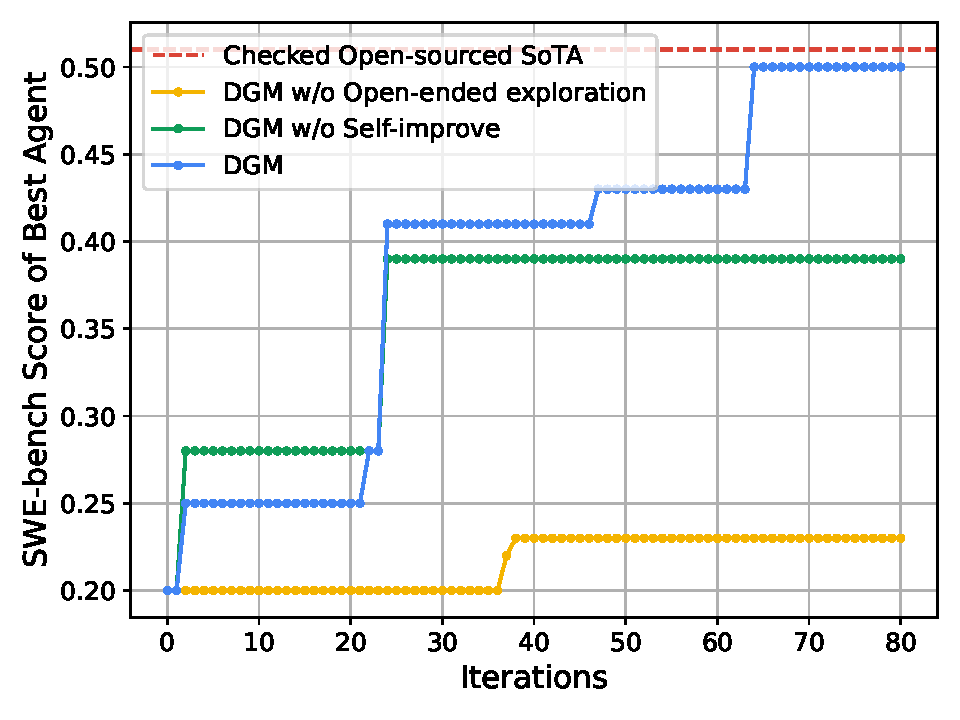
\includegraphics[width=\textwidth]{figures/dgm_comparisons.pdf}
        \label{fig:dgm-comparisons-swe}
    \end{subfigure}
    \hfill
    \begin{subfigure}[t]{0.48\textwidth}
        \centering
        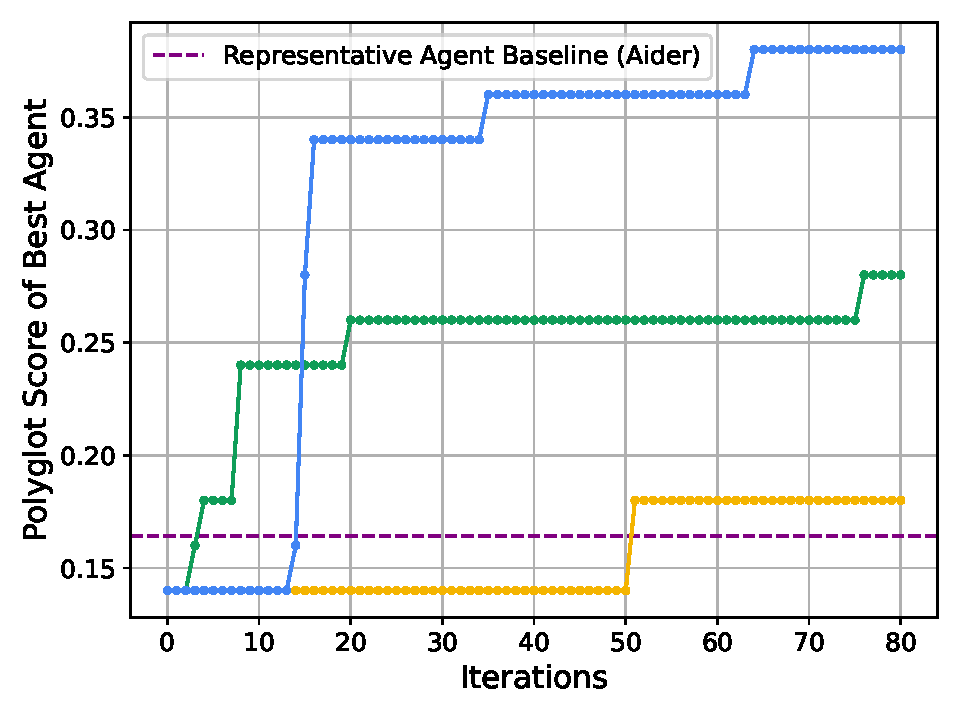
\includegraphics[width=\textwidth]{figures/dgm_comparisons_polyglot.pdf}
        \label{fig:dgm-comparisons-polyglot}
    \end{subfigure}
    % \vspace{-5mm}
    \caption{\textbf{Self-improvement and open-ended exploration enable the DGM to continue making progress and improve its performance.} The DGM automatically discovers increasingly better coding agents and performs better on both (Left) SWE-bench and (Right) Polyglot. It outperforms baselines that lack either self-improvement or open-ended exploration, showing that both components are essential for continual self-improvement. These scores are obtained from evaluating on the benchmark subsets detailed in \Cref{sec:benchmarks}.}
    \label{fig:dgm-comparisons}
    % \vspace{-3mm}
\end{figure}

\begin{figure}[ht]
    \centering
    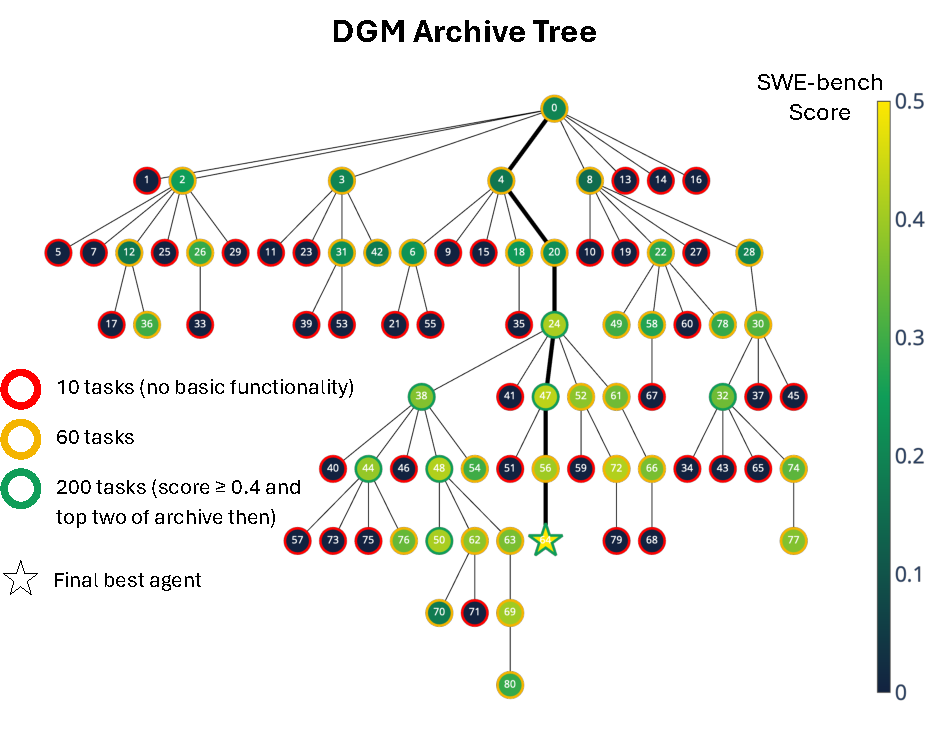
\includegraphics[width=0.45\textwidth]{figures/dgm_archive.pdf}
    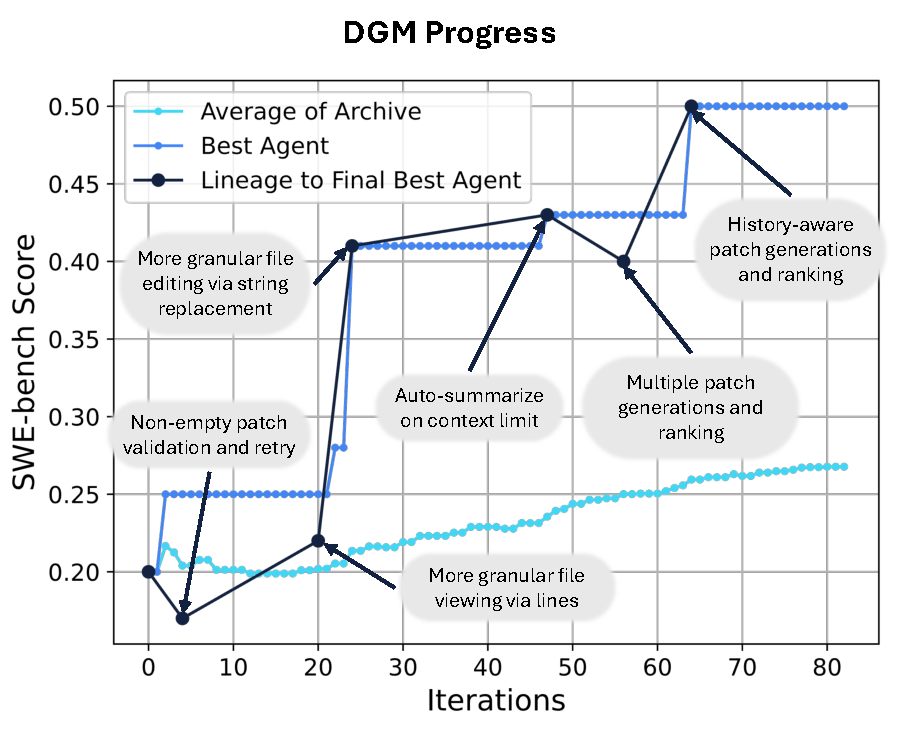
\includegraphics[width=0.45\textwidth]{figures/dgm_progress.pdf}
    % \vspace{-2mm}
    \caption{\textbf{The DGM automatically self-improves to become a better coding agent.} (Left) Archive of coding agents generated during the DGM run on SWE-bench. Each node represents a coding agent, with node 0 corresponding to the base agent. Node color indicates performance on SWE-bench (percentage of solved tasks), while border color reflects the number of tasks for which the agent was evaluated. Edges show which agents self-modified to produce the offsprings. Many paths to innovation traverse lower-performing nodes, and key innovations (like node 24) lead to an explosion of innovations built on top of them. Both properties underscore the benefits of open-ended search. (Right) Progress plot of the DGM on SWE-bench. The light blue line shows the average score of all agents possessing basic codebase-editing functionality. The blue line tracks the best score achieved by any agent in the archive at each iteration. The dark line shows the lineage of the final best-discovered agent and its precursor nodes, which includes two performance dips. This illustrates the benefits of open-ended search, which explores a diverse set of interesting stepping stones instead of focusing only on branching off the best solution found so far.}
    \label{fig:dgm-archive}
    \label{fig:dgm-progress}
    % \vspace{-6mm}
\end{figure}

After \DgmMainIterations{} iterations of the DGM, the coding agent's performance increases from \DgmSweBenchInitial{} to \DgmSweBenchFinal{} on SWE-bench, and from 14.0\% to 38.0\% on Polyglot (\Cref{fig:dgm-comparisons}). Since the DGM is evaluated on only 50 tasks in the Polyglot experiment setup (\Cref{sec:benchmarks}), we additionally evaluate both the base agent and the best DGM-discovered agent on the full Polyglot benchmark to more accurately estimate the improvement. On the full Polyglot benchmark, the DGM improves the coding agent from \DgmPolyglotInitial{} to \DgmPolyglotFinal{}. This shows that the DGM can automatically self-improve to create a better coding agent. Moreover, the performance of the best DGM-discovered agent is comparable to that of the checked, open-source, human-designed SoTA on SWE-bench (\Cref{fig:dgm-comparisons}). On Polyglot, although the DGM starts with a base agent whose performance is lower than that of Aider, it discovers an agent that far surpasses Aider (\Cref{fig:dgm-comparisons}). The DGM-discovered agents are comparable to or outperform handcrafted agents on both benchmarks. While the SoTA SWE-bench agent and Aider were painstakingly shaped by human efforts, the DGM hints at a future in which such ingenuity is automated, evolving through self-referential cycles of continuous self-improvements.

The DGM automatically improves both the tools and the workflow of how FMs are utilized (\Cref{fig:dgm-progress}). For example, the DGM enhanced the edit tool to allow more granular file viewing (by lines) and more precise file editing (by string replacement), instead of always viewing or replacing the entire file. Workflow improvements include making multiple attempts to solve a task and using another FM to evaluate and select the best solution. Other workflow improvements include considering previous attempts when generating subsequent ones. \Cref{app:best-agent-dgm} and \Cref{app:best-agent-dgm-polyglot} show all modifications leading up to the final best-discovered agents on SWE-bench and Polyglot respectively.

Because open-ended exploration allows branching from any agent in the archive with non-zero probability, the DGM can get out of deceptive dips or peaks in performance. For example, at iterations 4 and 56 of the experiment on SWE-bench, although the agent's score temporarily fell below that of its parent, the DGM was still able to explore innovations along that path and create a new agent that outperformed all of its predecessors (\Cref{fig:dgm-progress}). Furthermore, open-ended exploration allows different implementations of the same target functionality to be attempted. For example, while the goal is to provide finer‑grained editing tools, the specific implementation of this feature can vary greatly and hence lead to very different performance (\Cref{app:supp-dgm-diffimpl}). The DGM can explore multiple implementations to find the most suitable one and avoid getting trapped in a suboptimal one.

The DGM outperforms the baselines of DGM w/o self-improve and DGM w/o open-ended exploration on both benchmarks (\Cref{fig:dgm-comparisons}). Without updating the meta agent that modifies coding agents, DGM w/o self-improve improves the agents in early iterations, but its gains taper off quickly (\Cref{app:plots-swe}). In DGM w/o open-ended exploration, only the most recent agent is retained, so a poorly performing self-modification makes subsequent improvements harder to achieve (\Cref{app:plots-swe}).

\begin{figure}[ht]
    \centering
    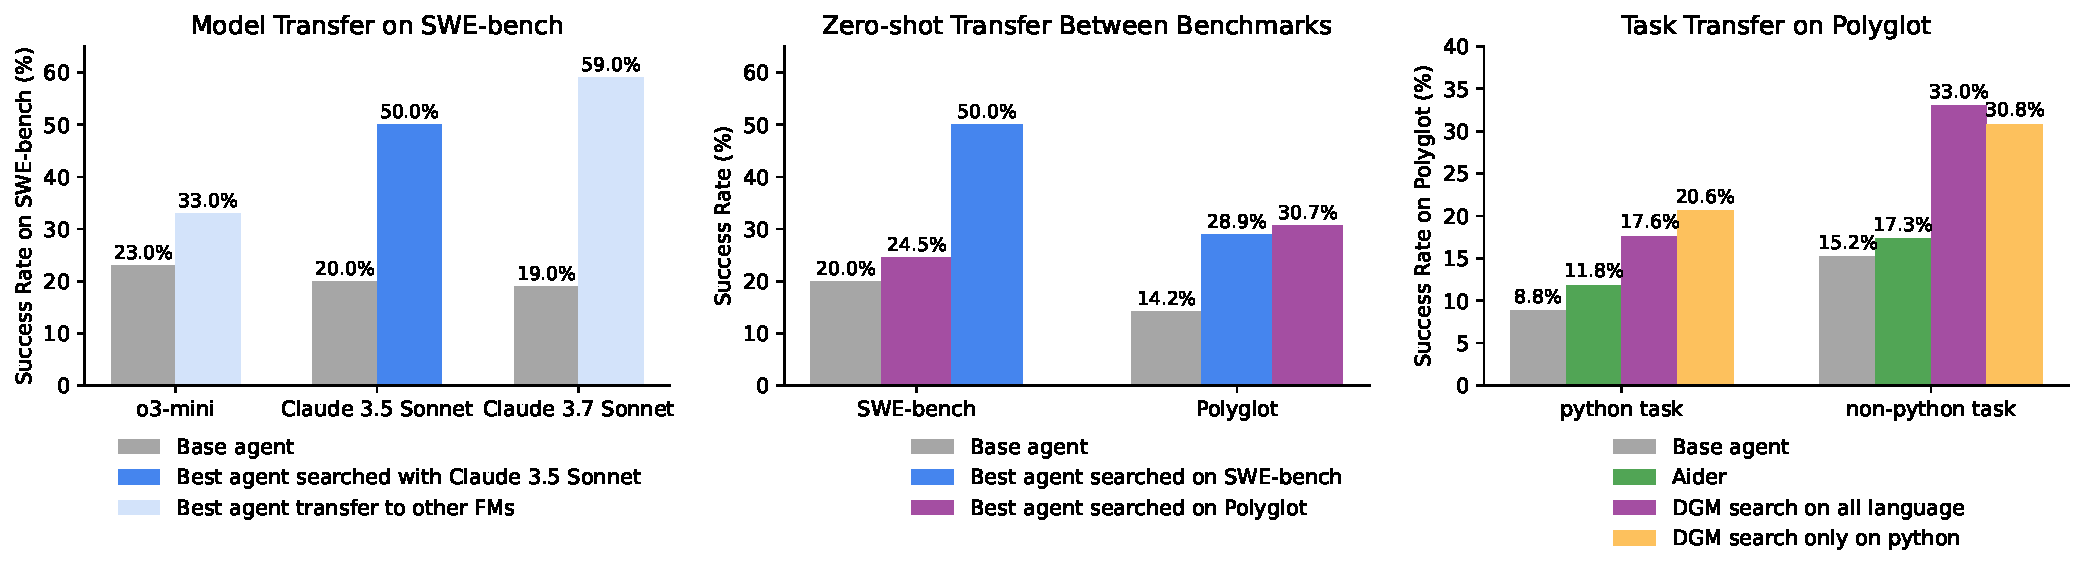
\includegraphics[width=0.95\textwidth]{figures/transfer_model_task.pdf}
    % \vspace{-3mm}
    \caption{\textbf{Transfer between Models, Benchmarks, and Tasks.} The superior performance of DGM-discovered agents can be transferred across (Left) different models, (Middle) benchmarks, and (Right) different programming language tasks in Polyglot, such as from Python tasks to C++ tasks.}
    \label{fig:transfer-overview}
    % \vspace{-4mm}
\end{figure}

To evaluate the generality of the improvements from the DGM, we tested the base agent (\Cref{sec:experiment-setup}) and the best agent discovered during the DGM run (\Cref{fig:dgm-comparisons}) with different FMs than those used during optimization. For SWE-bench, where the DGM was run using Claude 3.5 Sonnet (New), we replaced the FM with Claude 3.7 Sonnet~\citep{anthropic2025claude37} or o3-mini, and evaluated on 200 tasks (\Cref{fig:transfer-overview}, Left). With o3-mini, the base agent achieved 23.0\% and the DGM-discovered agent 33.0\%. With Claude 3.7 Sonnet, the base agent achieved 19.0\% and the DGM-discovered agent 59.5\%. These results suggest that the DGM yields improvements that generalize across FMs, rather than being tightly coupled to the specific FM used during its run (\Cref{fig:transfer-overview}). Model transfer results on Polyglot are presented in \Cref{app:polyglot-model}.

Furthermore, we investigate the transferability of the DGM-discovered agent across different benchmarks and programming languages. First, we evaluate the best DGM-discovered agent from one benchmark (e.g., SWE-bench) on a completely held-out benchmark (e.g., Polyglot), and vice versa (\Cref{fig:transfer-overview}, Middle). The best agent evolved on SWE-bench achieves 28.9\% on Polyglot, compared to the initial agent's baseline of 14.2\%. Conversely, the best agent evolved on Polyglot achieves 24.5\% on SWE-bench, outperforming the original baseline of 20.0\%. Since each agent was optimized without ever accessing the alternate benchmark, these evaluations represent truly held-out tests. The consistent performance gains across benchmarks support our claim that DGM's improvements reflect general skill acquisition rather than overfitting or exploitation of benchmark-specific artifacts. Second, we experiment with a version of the DGM trained exclusively on Python tasks from Polyglot and then transfer the discovered agent to tasks in other languages. Focusing primarily on Python tasks slightly improves performance on Python tasks but reduces performance on non-Python tasks compared to the DGM trained on all languages (\Cref{fig:transfer-overview}, Right). However, after being transferred from Python to other unseen languages during the search, the agent still achieves performance comparable to that of the DGM trained on all languages and substantially outperforms both the base agent and Aider. These results demonstrate the robustness of the discovered improvements, showing that they do not overfit to a specific programming language. We also present additional results in \Cref{app:add-results}.

% \vspace{-2mm}
